\documentclass{beamer}
\usetheme[block=fill]{metropolis}

\usepackage[english]{babel}
%\usepackage[utf8]{inputenc}

% For notes
\usepackage{pgfpages}
\setbeameroption{show notes on second screen=right}
\usepackage{appendixnumberbeamer} % don't number the backup slides

\usepackage{amsmath,amssymb} % math
\usepackage{graphicx} % images
\DeclareGraphicsExtensions{.eps,.pdf,.png,.jpg,.gif,.jpeg}
\graphicspath{{./img/}}
\usepackage[export]{adjustbox}

\title{AURsec \newline Detecting and preventing targeted attacks in the Arch User Repository: A blockchain-based approach}
\author{Lukas Krismer \& Bennett Piater}
\institute{Universität Innsbruck - QE - Christian Sillaber}
\date{\today}

\begin{document}

\maketitle


\begin{frame}
	\frametitle{Outline}
	\tableofcontents
	\note{1 min L | }
	\note{Betreuer: Christian Sillaber - Quality Engineering}
\end{frame}




\section{Background: AUR}

\begin{frame}{AUR}
	\pause
	\begin{itemize}
		\item \textbf{AUR}=\alert{A}rch Linux \alert{U}ser \alert{R}epository
		\item Contains package build scripts (PKGBUILDs)
		\item Packages can be voted for inclusion in the official repositories
		\item Easy to use using so-called AUR helpers
		\item Everybody can upload PKGBUILDs
		\item Anyone can adopt orphaned packages
	\end{itemize}
	\note{3 min L | Arch has a active community -> packages to ftp://ftp.archlinux.org/income (long delay) -> Trusted User Repo -> AUR
	Comparable to Pypi npm | fulfill conditions }
\end{frame}

\begin{frame}[t]{Threat Assessment}
	\begin{columns}
		\column{\dimexpr\paperwidth}
		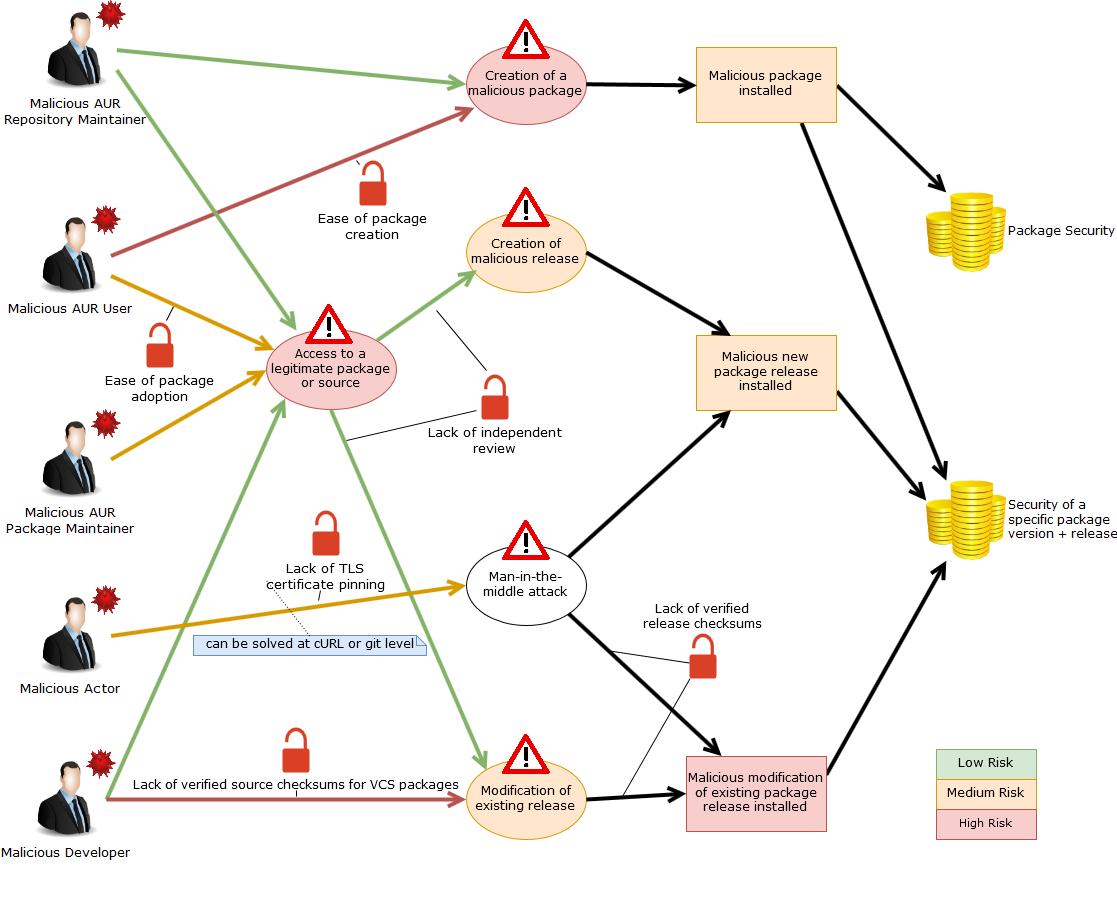
\includegraphics[width=0.98\paperwidth,height=0.9\paperheight,left]{threat1n.png}
	\end{columns}
	\note{3.5 min B |

	\emph{Explain the main security issues!}
	\begin{itemize}
		\item The underlying problems of the AUR are not really solvable
		\item Too many people have access to build scripts and sources
		\item \rightarrow:~~(automated) server-side signatures would only prevent MITM
		\item malicious packages, releases and modifications of releases are very easy to do
	\end{itemize}}
\end{frame}

\section{Our Project}

\begin{frame}{Covered Threats}
	\begin{columns}
		\column{\dimexpr\paperwidth}
		\includegraphics<1>[width=0.98\paperwidth,height=0.9\paperheight,left]{threat1n.png}
		\includegraphics<2>[width=0.98\paperwidth,height=0.9\paperheight,left]{threat2n.png}
	\end{columns}
	\note{2 min L | }
\end{frame}

\begin{frame}[standout]
	Live Demo
	\note{4 min BL | Wirklich live

	git clone aur:aursec \\
	aursec-hash -d aursec \\
	aursec-hash aursec | aursec-verify-hashes \\
	aursec -v aursec \\
	echo var=val >> aursec/PKGBUILD \\
	aursec aursec

	?? \\
	git clone aur:aursec-git \\
	aursec -d aursec-git \\
	}
\end{frame}

\section{Implementation Details}


\begin{frame}{Blockchain}
	\begin{itemize}
		\item is a secure, distributed database
		\item Used by Cryptocurrency
		\item keywords: transaction, miner, smart contract
		\item Ethereum \& Solidity our means of choice
	\end{itemize}
	\note{4 min L | Cryptocurrency }
\end{frame}

\begin{frame}{Workflow}

	\begin{columns}
		\column{\dimexpr\paperwidth}
		\includegraphics<1,3>[width=0.98\paperwidth,height=0.9\paperheight,left]{Workflow2}
		\begin{center}
		\includegraphics<2>[width=0.9\paperwidth]{decision}
		\end{center}
		%\includegraphics<3>[width=0.98\paperwidth,height=0.9\paperheight,left]{Workflow2}
	\end{columns}
	\note{3 min B | }
	\note{}
\end{frame}

\begin{frame}{Components}
	\note{4 min BL |

	UNIX philosophy - small tools doing one thing well.
	Work on stdin/stdout with blocking I/O.

	Good parallelism, straightforward to maintain and extend
	}

	\begin{block}{Main Pipeline}
		\begin{itemize}
		\item \texttt{aursec} (state machine)
		\item \texttt{aursec-hash} (generate ID and hash)
		\item \texttt{aursec-verify-hashes} (blockchain interaction)
		\item smart contract
		\end{itemize}
	\end{block}
	\pause
	\begin{block}{Other Tools}
	\begin{itemize}
		\item \texttt{aursec-chain}
		\item Systemd services and timers
	\end{itemize}
	\end{block}
\end{frame}

\begin{frame}{Extensions}
	\begin{itemize}
		\item ZSH completion
		\item Integration into aurutils
		\item Terminal User-Interface
	\end{itemize}
	\note{2 min L | Live Demo

	aursec-tui \\
	aurutils integration}
\end{frame}


\section{Comparison and Summary}
\begin{frame}{Comparison with other approaches}
	\note{2 min B |

	Custom repositories make sense for private organizations -- not for large scale

	Redesigning the AUR is not an option -- no one wants to sacrifice the ease of use

	\rightarrow~~ AURsec seems like overkill, but it's still the best solution available.}

	\begin{block}{Disadvantages of our approach}
		\begin{itemize}
			\item Local blockchain copy (disk space)
			\item Synchronization (background process)
			\item Mining difficulty (computationally expensive)
		\end{itemize}
	\end{block}

	\pause
	\begin{block}{Alternative: Database + Web service}
		\begin{itemize}
			\item Light-weight (no local blockchain, no mining)
			\item Single point of trust
		\end{itemize}
	\end{block}

	\pause
	\begin{block}{Other Options:}
		\begin{itemize}
			\item Create a new, trusted source or binary repository downstream of the AUR (manual auditing)
			\item Completely redesign the AUR
		\end{itemize}
	\end{block}
\end{frame}

% We won't necessarily do this
% \begin{frame}{Lessons Learned}
% 	\begin{itemize}
% 		\item bash % Think like in FP for the structure (streams and pipelines); static checking against syntactic pitfalls; invent appropriate testing system where possible/applicable
% 		\item solidity % good abstraction, easy; does what we want in the background
% 		\item urwid
% 		\item JSON-RPC
% 	\end{itemize}
% 	\note{2 min BL | }
% \end{frame}

\begin{frame}{Planned Improvements}
	\begin{block}{Smart Contract Improvement}
		Also remember second-most-common hash.
		Allows taking ratio into account instead of simple threshold.
	\end{block}

	\pause
	\begin{block}{Mining Improvements}
		\begin{itemize}
			\item Tweak difficulty (need more testing) % not easy to manipulate, but usable
			\item Periodic mining using set time (effort) instead of block count % Better for fairness
			\item Defer periodic mining if on battery power
		\end{itemize}
	\end{block}
	\note{2 min B | }
\end{frame}


\begin{frame}{Schedule}
	\begin{itemize}
		\item \textbf{25.10} \emph{prototype:} hashing \hfill B
		\item \textbf{08.11} \alert{Initial Presentation}\hfill L
		\item \textbf{15.11} \emph{prototype:} library without blockchain back-end \hfill B/L
		\item \textbf{15.11} Bash-API for the blockchain \hfill L
		\item \textbf{30.11} \emph{finish:} \alert{Solidity program} \hfill B
		\item \textbf{08.12} deploy local blockchain for development \hfill L
		\item \textbf{08.12} running server with ethereum-node \hfill B/L
		\item \textbf{15.12} \emph{prototype:} \alert{Library} incl. back-end \hfill L
		\item \textbf{20.12} \emph{contrib:} pre-build-hooks in aurutils \hfill B
	\end{itemize}
	\note{2 min B

	Wir haben eine sehr \textbf{detaillierte Planung} ausgearbeitet.
	Einerseits benötigen wir sie, um effizient \textbf{kooperieren} zu können und zügig voran zu kommen; Andererseits soll sie uns auch ein Maximaltempo vergeben, denn wir tendieren beide eher dazu, uns zu \textbf{überarbeiten}.

	\begin{itemize}
		\item Solidity-program auf Blockchain
		\item Library-Prototyp
		\item Beiträge zum AUR-Helper aurutils über Weihnachten
	\end{itemize}
	}
\end{frame}

\begin{frame}{Schedule}
	\begin{itemize}
		\item \textbf{10.01} \emph{contrib:} TLS-public-key-pinning in aurutils \hfill B
		\item \textbf{10.01} configuration and trust-cutoff \hfill L
		\item \textbf{15.01} \emph{test:} \alert{Integration in aurutils} \hfill B
		\item \textbf{15.02} \alert{AUR package} incl. private blockchain \hfill B
		\item \textbf{01.03} \emph{finish:} libary and aurutils-Hook \hfill B
		\item \textbf{31.03} \emph{finish:} Web- and/or CLI-Interface \hfill L
		\item \textbf{21.04} \alert{Draft paper} for feedback\hfill
		\item \textbf{??.05} \emph{finish:} Paper\hfill
		\item \textbf{??.05} Final presentation\hfill L
	\end{itemize}
	\note{2 min B

	\begin{itemize}
		\item am 15.01 mit aurutils testbar
		\item AUR-Paket zur einfachen Verbreitung
		\item Programmierung endet am 31. März
		\item Meiste Schreibarbeit im April und besonders über Ostern
		\item Abgabe bequem for den Klausuren
	\end{itemize}}
\end{frame}

\begin{frame}{Schedule}
	\begin{columns}
		\column{\dimexpr\paperwidth}
		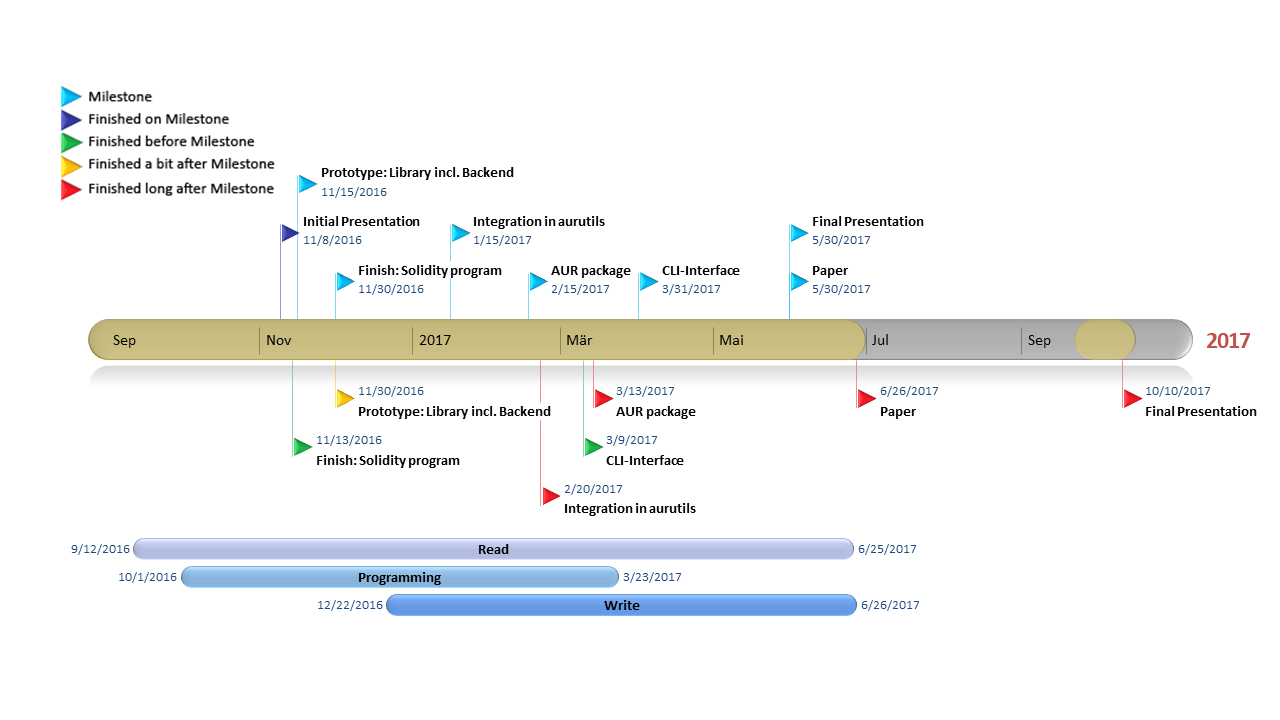
\includegraphics[width=0.9\paperwidth]{timeline}
	\end{columns}
	\note{2 min L | }
\end{frame}

\begin{frame}[standout]
	Questions?
\end{frame}


\end{document}
